% Provenance (never printed): cycle 2 "Questionner le monde de la matiere"
% (solid materials, observing and sorting) and cycle 3 theme 4 (local geology,
% rocks for building); see sources/book1/PROVENANCE.md. Book 1, grade 3, ch. 1.
\chapter{पत्थर, कंकड़ और रेत}\label{ch:g3:stones-pebbles-sand}

टॉम छुट्टियों में एक \omterm{def:g1:landscapes-around-us:water}{नदी} के किनारे है। \omterm{def:g3:stones-pebbles-sand:pebble}{बजरी} वाले किनारे पर, जहाँ पानी उथला
है, वह एक \omterm{def:g3:stones-pebbles-sand:pebble}{कंकड़} उठाता है। वह चिकना और गोल है, लगभग अंडे जैसा, और उसकी
मुट्ठी में समा जाता है। पिछले हफ़्ते, उसी \omterm{def:g1:landscapes-around-us:landform}{घाटी} में बहुत ऊपर एक \omterm{def:g1:landscapes-around-us:landform}{पहाड़ी}
रास्ते पर अपने माता-पिता के साथ चलते हुए, उसने एक पथरीली ढलान के नीचे उसी
रंग के पत्थर पड़े देखे थे --- पर वे पत्थर नुकीले थे, किनारों और कोनों वाले।

\omterm{def:g1:landscapes-around-us:landform}{पर्वत} का एक नुकीला पत्थर नीचे \omterm{def:g1:landscapes-around-us:landform}{घाटी} में चिकना, गोल \omterm{def:g3:stones-pebbles-sand:pebble}{कंकड़} कैसे बन गया? यह
जानने के लिए, आओ ख़ुद \omterm{def:g3:stones-pebbles-sand:rock}{चट्टान} से शुरू करें।

\begin{omfigure}
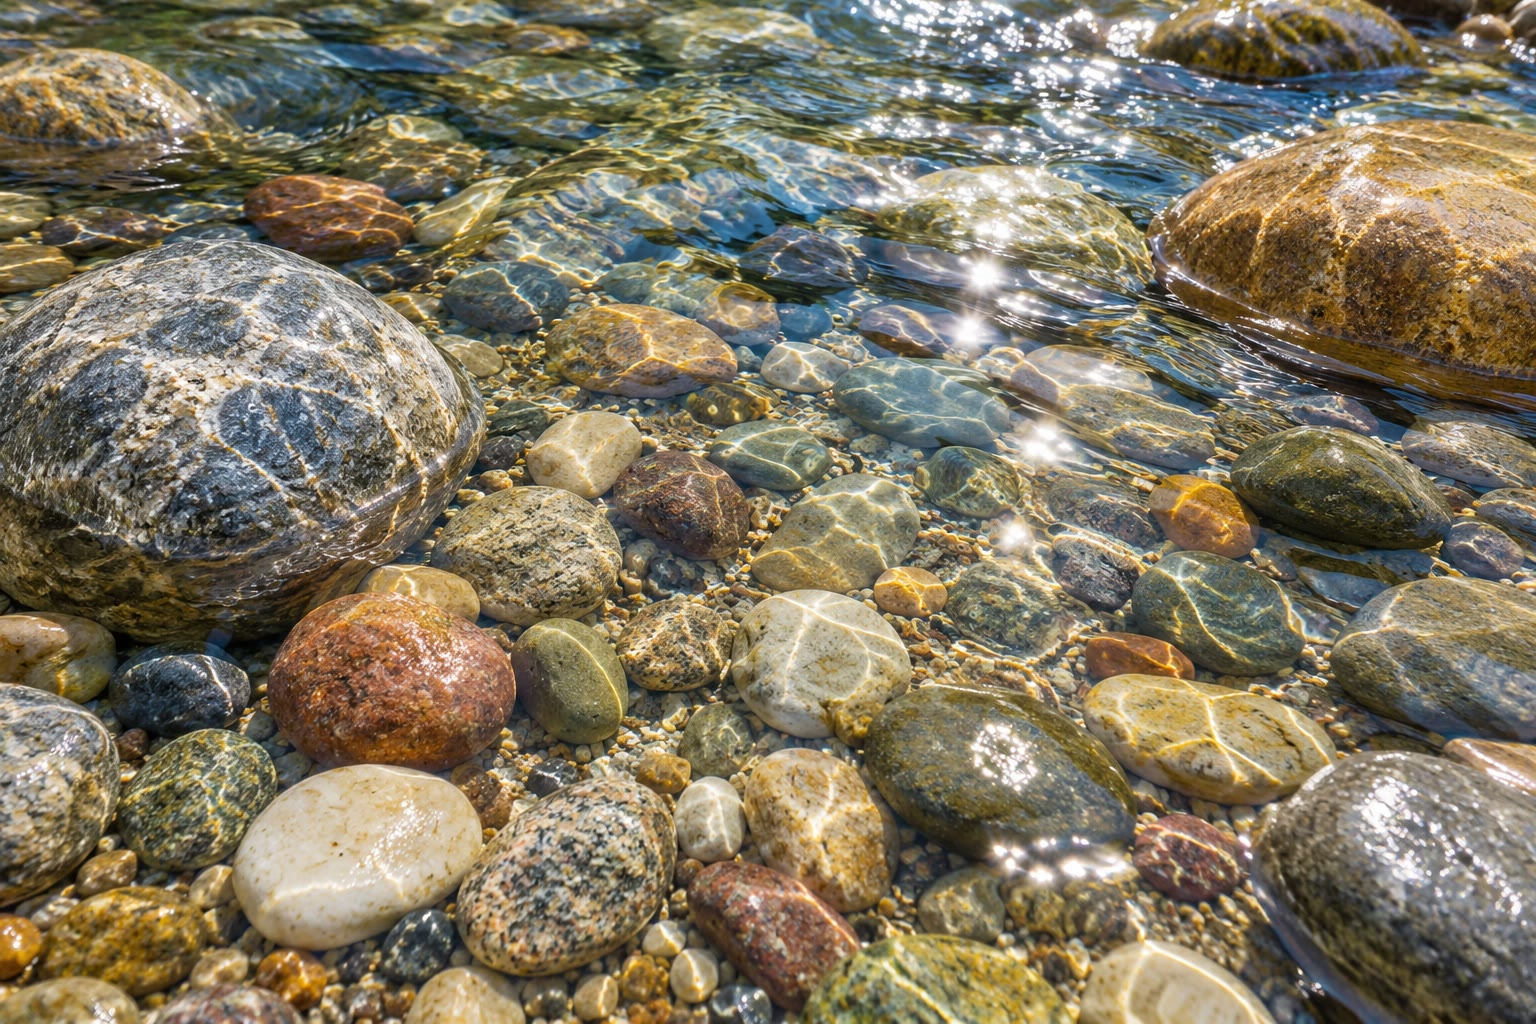
\includegraphics[width=0.62\linewidth]{images/book1/ai/g3-stream-pebbles.jpg}

{\small एक नाले के साफ़ पानी के नीचे गोल \omterm{def:g3:stones-pebbles-sand:pebble}{कंकड़}।}
\end{omfigure}

\begin{recall}
\omterm{def:g1:landscapes-around-us:landscape}{भूदृश्य} में \omterm{def:g1:landscapes-around-us:landform}{पर्वत}, \omterm{def:g1:landscapes-around-us:landform}{पहाड़ियाँ}, \omterm{def:g1:landscapes-around-us:landform}{घाटियाँ} और \omterm{def:g1:landscapes-around-us:landform}{मैदान} होते हैं, और \omterm{def:g1:landscapes-around-us:water}{नदियाँ} जो ऊँची
ज़मीन से नीचे \omterm{def:g2:water-on-earth:ocean}{समुद्र} की ओर बहती हैं (\cref{ch:g1:landscapes-around-us})।
ज़मीन की सबसे ऊपरी परत, जिसमें पौधे उगते हैं, मिट्टी है: सजीव उसे कैसे
बनाते हैं, यह जीवविज्ञान की पुस्तकें बताती हैं।
\end{recall}

\section{चट्टान: हमारे पैरों के नीचे की कठोर ज़मीन}

किसी बग़ीचे में एक गहरा गड्ढा खोदो। पहले तुम्हें गहरे रंग की, नरम मिट्टी
मिलती है जिसमें जड़ें हैं। उसके नीचे मिट्टी हल्के रंग की और ज़्यादा पथरीली
हो जाती है। और अगर तुम काफ़ी गहरा खोद पाते, तो तुम हमेशा किसी ऐसी कठोर
चीज़ तक पहुँचते जिसे फावड़ा काट नहीं सकता: \omterm{def:g3:stones-pebbles-sand:rock}{चट्टान}।

\begin{definition}[चट्टान और आधार चट्टान]\label{def:g3:stones-pebbles-sand:rock}
\emph{चट्टान}\index{चट्टान} एक कठोर, प्राकृतिक पदार्थ है जिससे ठोस पृथ्वी
बनी है। \emph{आधार चट्टान}\index{आधार चट्टान} वह ठोस चट्टान है जो ज़मीन पर
हर जगह मिट्टी के नीचे, और समुद्री तल की \omterm{def:g3:stones-pebbles-sand:sand}{रेत} और \omterm{def:g3:stones-pebbles-sand:sand}{कीचड़} के नीचे फैली है।
\end{definition}

ज़्यादातर जगहों पर \omterm{def:g3:stones-pebbles-sand:rock}{आधार चट्टान} मिट्टी, घास और पेड़ों के नीचे छिपी रहती है।
हम उसे वहाँ देखते हैं जहाँ उसे ढकने के लिए मिट्टी नहीं है: \omterm{def:g1:landscapes-around-us:landform}{पर्वतों} की खड़ी
ढलानों में, \omterm{def:g2:water-on-earth:ocean}{समुद्र} के किनारे की ऊँची खड़ी \omterm{def:g3:stones-pebbles-sand:rock}{चट्टानों} में, और \omterm{def:g1:landscapes-around-us:landform}{पहाड़ी} को काटकर
बनाई गई सड़कों के किनारे।

\begin{omfigure}
\begin{tikzpicture}[x=1cm, y=1cm, font=\small]
  % bedrock
  \fill[omLithGranite!60] (0,0) rectangle (11,2.2);
  \foreach \x/\y in {0.6/0.5, 1.8/1.4, 3.1/0.7, 4.4/1.6, 5.6/0.4, 6.9/1.2, 8.3/0.6, 9.6/1.5, 10.3/0.4}
    \draw[black!40, line width=0.4pt] (\x,\y) -- ++(0.5,0.25);
  % soil (thick on the left, missing on the steep right)
  \fill[brown!55] (0,2.2) -- (0,3.4) .. controls (2,3.5) and (4,3.4) .. (5.6,3.2) -- (6.4,2.9) -- (6.4,2.2) -- cycle;
  \fill[brown!30] (0,2.2) rectangle (6.4,2.65);
  % rock showing on the right: a hill side with no soil
  \fill[omLithGranite!60] (6.4,2.2) -- (6.4,2.9) -- (7.6,3.9) -- (8.8,4.3) -- (11,4.3) -- (11,2.2) -- cycle;
  \draw[black!60] (0,3.4) .. controls (2,3.5) and (4,3.4) .. (5.6,3.2) -- (6.4,2.9) -- (7.6,3.9) -- (8.8,4.3) -- (11,4.3);
  % grass and roots
  \foreach \x in {0.3,0.8,...,5.3}
    \draw[green!50!black, line width=0.6pt] (\x,{3.4-0.04*\x}) -- ++(0.05,0.18);
  \foreach \x in {1.2,3.4,4.9}
    \draw[brown!80!black, line width=0.5pt] (\x,3.3) -- ++(-0.1,-0.5) -- ++(0.15,-0.3);
  % labels
  \node[anchor=west] at (11.2,3.6) {सतह पर दिखती};
  \node[anchor=west] at (11.2,3.2) {चट्टान};
  \draw[black!60] (11.15,3.4) -- (9.6,4.15);
  \node[anchor=east] at (-0.2,2.9) {मिट्टी};
  \draw[black!60] (-0.15,2.9) -- (0.6,2.9);
  \node[anchor=west] at (11.2,1.1) {आधार चट्टान};
  \draw[black!60] (11.15,1.1) -- (10.6,1.1);
\end{tikzpicture}

{\small ज़मीन का एक कटा हुआ दृश्य। मिट्टी के नीचे हमेशा ठोस \omterm{def:g3:stones-pebbles-sand:rock}{आधार चट्टान} होती
है। दाईं ओर की खड़ी \omterm{def:g1:landscapes-around-us:landform}{पहाड़ी} ढलान पर मिट्टी नहीं है और \omterm{def:g3:stones-pebbles-sand:rock}{चट्टान} सतह पर दिखती है।}
\label{fig:g3:stones-pebbles-sand:ground}
\end{omfigure}

\section{चट्टान से कंकड़ तक}

\omterm{def:g3:stones-pebbles-sand:rock}{चट्टान} कठोर होती है, पर वह हमेशा नहीं टिकती। सर्दियों में पानी \omterm{def:g3:stones-pebbles-sand:rock}{चट्टान} की
दरारों में घुस जाता है, जम जाता है और फैलता है, और दरारों को चौड़ा कर देता
है। जड़ें भी दरारों में उग आती हैं। धीरे-धीरे टुकड़े टूटकर गिरते हैं: \omterm{def:g1:landscapes-around-us:landform}{पर्वतों}
की ढलानों के नीचे पड़े नुकीले पत्थर यहीं से आते हैं।

जब कोई नुकीला पत्थर किसी \omterm{def:g1:landscapes-around-us:landform}{पहाड़ी} नाले में गिरता है, तो पानी उसे तली पर
लुढ़काता है, दूसरे पत्थरों से टकराता है, और \omterm{def:g3:stones-pebbles-sand:sand}{रेत} पर घसीटता है। सबसे पहले
उसके कोने घिसते हैं। वह जितनी दूर जाता है, उतना ही गोल और चिकना होता जाता
है। निचली \omterm{def:g1:landscapes-around-us:landform}{घाटी} तक पहुँचते-पहुँचते वह \omterm{def:g3:stones-pebbles-sand:pebble}{कंकड़} बन चुका होता है।

\begin{definition}[कंकड़ और बजरी]\label{def:g3:stones-pebbles-sand:pebble}
\emph{कंकड़}\index{कंकड़} \omterm{def:g3:stones-pebbles-sand:rock}{चट्टान} का एक छोटा टुकड़ा है जिसे \omterm{def:g1:landscapes-around-us:water}{नदी} में या \omterm{def:g2:water-on-earth:ocean}{समुद्र}
\omterm{def:g1:landscapes-around-us:water}{तट} पर पानी ने लुढ़का-लुढ़काकर गोल और चिकना कर दिया है। \emph{बजरी}\index{बजरी}
एक साथ पड़े छोटे पत्थरों और कंकड़ों का ढेर है, जिसके कण \omterm{def:g3:stones-pebbles-sand:sand}{रेत} के कणों से बड़े
होते हैं।
\end{definition}

\begin{omfigure}
\begin{tikzpicture}[x=1cm, y=1cm, font=\small]
  \draw[ocBlue!70!black, line width=1.2pt, -{Stealth[length=3mm]}] (0,0) -- (12.2,0);
  \node[below, font=\scriptsize] at (6.1,-0.15) {नाला पत्थर को ढलान पर नीचे ले जाता है, हर बाढ़ में थोड़ा और आगे};
  \foreach \x/\shape/\t in {
     0.8/{(-0.55,-0.1) -- (-0.2,0.5) -- (0.35,0.55) -- (0.6,0.05) -- (0.3,-0.45) -- (-0.35,-0.5) -- cycle}/चट्टान से गिरा,
     4.0/{(-0.5,-0.1) [rounded corners=4pt] -- (-0.2,0.45) -- (0.3,0.5) -- (0.55,0.05) -- (0.3,-0.4) -- (-0.35,-0.45) -- cycle}/कोने घिसे,
     7.2/{(-0.45,-0.05) [rounded corners=8pt] -- (-0.15,0.42) -- (0.3,0.45) -- (0.5,0.05) -- (0.3,-0.35) -- (-0.3,-0.4) -- cycle}/ज़्यादा गोल और छोटा,
     10.4/{(0,0) ellipse (0.45 and 0.3)}/एक चिकना कंकड़} {
    \begin{scope}[shift={(\x,1.1)}]
      \fill[omLithGranite!80, draw=black!70] \shape;
    \end{scope}
    \node[font=\scriptsize] at (\x,0.35) {\t};
  }
\end{tikzpicture}

{\small \omterm{def:g1:landscapes-around-us:water}{नदी} में एक पत्थर की यात्रा: \omterm{def:g3:stones-pebbles-sand:rock}{चट्टान} से गिरते समय नुकीला, धारा के साथ
लंबी यात्रा के बाद गोल और चिकना।}
\label{fig:g3:stones-pebbles-sand:journey}
\end{omfigure}

\begin{remark}[पत्थर का आकार पढ़ना]\label{rem:g3:stones-pebbles-sand:shape}
पत्थर का आकार हमें उसकी कहानी बताता है। नुकीला पत्थर उस \omterm{def:g3:stones-pebbles-sand:rock}{चट्टान} से ज़्यादा
दूर नहीं गया है जिससे वह टूटा था। गोल, चिकने \omterm{def:g3:stones-pebbles-sand:pebble}{कंकड़} को पानी ने, \omterm{def:g1:landscapes-around-us:water}{नदी} में या
\omterm{def:g2:water-on-earth:ocean}{समुद्र} की लहरों में, बहुत समय तक लुढ़काया है।
\end{remark}

\section{रेत और कीचड़}

एक-दूसरे से टकराने वाले पत्थर और \omterm{def:g3:stones-pebbles-sand:pebble}{कंकड़} नन्हे टुकड़े भी झाड़ते हैं। बहुत लंबे
समय में ये नन्हे टुकड़े \omterm{def:g3:stones-pebbles-sand:sand}{रेत} बन जाते हैं। \omterm{def:g3:stones-pebbles-sand:sand}{रेत} को आवर्धक लेंस से देखो: हर कण
\omterm{def:g3:stones-pebbles-sand:rock}{चट्टान} का या किसी सीप का एक छोटा-सा टुकड़ा है, अक्सर वह भी गोल।

\begin{definition}[रेत और कीचड़]\label{def:g3:stones-pebbles-sand:sand}
% ledger: usgs:wentworth
\emph{रेत}\index{रेत} टूटी \omterm{def:g3:stones-pebbles-sand:rock}{चट्टान} के खुले कणों से बनी है जो 2 मिलीमीटर से
छोटे होते हैं: हम हर कण को अब भी देख सकते हैं। \emph{कीचड़}\index{कीचड़}
इतने छोटे कणों से बना है कि हम उन्हें एक-एक करके नहीं देख सकते; गीला होने
पर वह नरम और चिपचिपा होता है।
\end{definition}

भूवैज्ञानिक \omterm{def:g3:stones-pebbles-sand:rock}{चट्टान} के टूटे टुकड़ों को आकार के हिसाब से छाँटते हैं, सबसे
बड़े से सबसे छोटे तक: शिलाखंड, \omterm{def:g3:stones-pebbles-sand:pebble}{कंकड़} और \omterm{def:g3:stones-pebbles-sand:pebble}{बजरी}, \omterm{def:g3:stones-pebbles-sand:sand}{रेत}, और \omterm{def:g3:stones-pebbles-sand:sand}{कीचड़}।

\begin{omfigure}
\begin{tikzpicture}[x=1mm, y=1mm, font=\small]
  % true size: 1 unit = 1 mm
  \draw[black!40] (0,-14) -- (150,-14);
  \foreach \x in {0,10,...,150} \draw[black!40] (\x,-14) -- (\x,-12.5);
  \foreach \x in {0,50,100,150} \node[font=\scriptsize, below] at (\x,-14.5) {\pgfmathparse{int(\x/10)}\pgfmathresult\,cm};
  % mud: too small
  \node[font=\scriptsize, align=center] at (6,14) {कीचड़};
  \fill[brown!60] (6,0) circle (0.05);
  \node[font=\scriptsize, align=center] at (6,4.5) {इतने छोटे कण\\कि दिखते नहीं};
  % sand grains: up to 2 mm
  \node[font=\scriptsize] at (28,14) {रेत};
  \foreach \x/\r in {22/0.3, 25/0.5, 28/0.75, 32/1.0}
    \fill[yellow!60!brown, draw=black!50, line width=0.2pt] (\x,0) circle (\r);
  \node[font=\scriptsize, align=center] at (28,5) {2 मिलीमीटर\\से छोटे};
  % gravel and pebbles
  \node[font=\scriptsize] at (78,22) {बजरी और कंकड़};
  \fill[omLithGranite!80, draw=black!60] (52,0) ellipse (2 and 1.5);
  \fill[black!25, draw=black!60] (62,0) ellipse (4 and 3);
  \fill[omLithGranite!80, draw=black!60] (78,0) ellipse (8 and 6);
  \fill[black!30, draw=black!60] (104,0) ellipse (15 and 10);
  % boulder: off scale
  \node[font=\scriptsize] at (138,22) {शिलाखंड};
  \fill[black!20, draw=black!60] (128,-10) .. controls (127,8) and (135,16) .. (142,15) .. controls (150,14) and (152,4) .. (149,-10) -- cycle;
  \node[font=\scriptsize, align=center, fill=white, fill opacity=0.7, text opacity=1, inner sep=1pt] at (139,4) {बहुत छोटा\\बनाया गया};
\end{tikzpicture}

{\small टूटी \omterm{def:g3:stones-pebbles-sand:rock}{चट्टान} के कण, सबसे छोटे से सबसे बड़े तक। \omterm{def:g3:stones-pebbles-sand:sand}{कीचड़}, \omterm{def:g3:stones-pebbles-sand:sand}{रेत}, \omterm{def:g3:stones-pebbles-sand:pebble}{बजरी} और
\omterm{def:g3:stones-pebbles-sand:pebble}{कंकड़} अपने असली आकार में बनाए गए हैं: किसी पैमाने से मिलाकर देखो।
शिलाखंड किसी कुर्सी जितना बड़ा हो सकता है, या किसी घर जितना।}
\label{fig:g3:stones-pebbles-sand:sizes}
\end{omfigure}

\begin{omfigure}
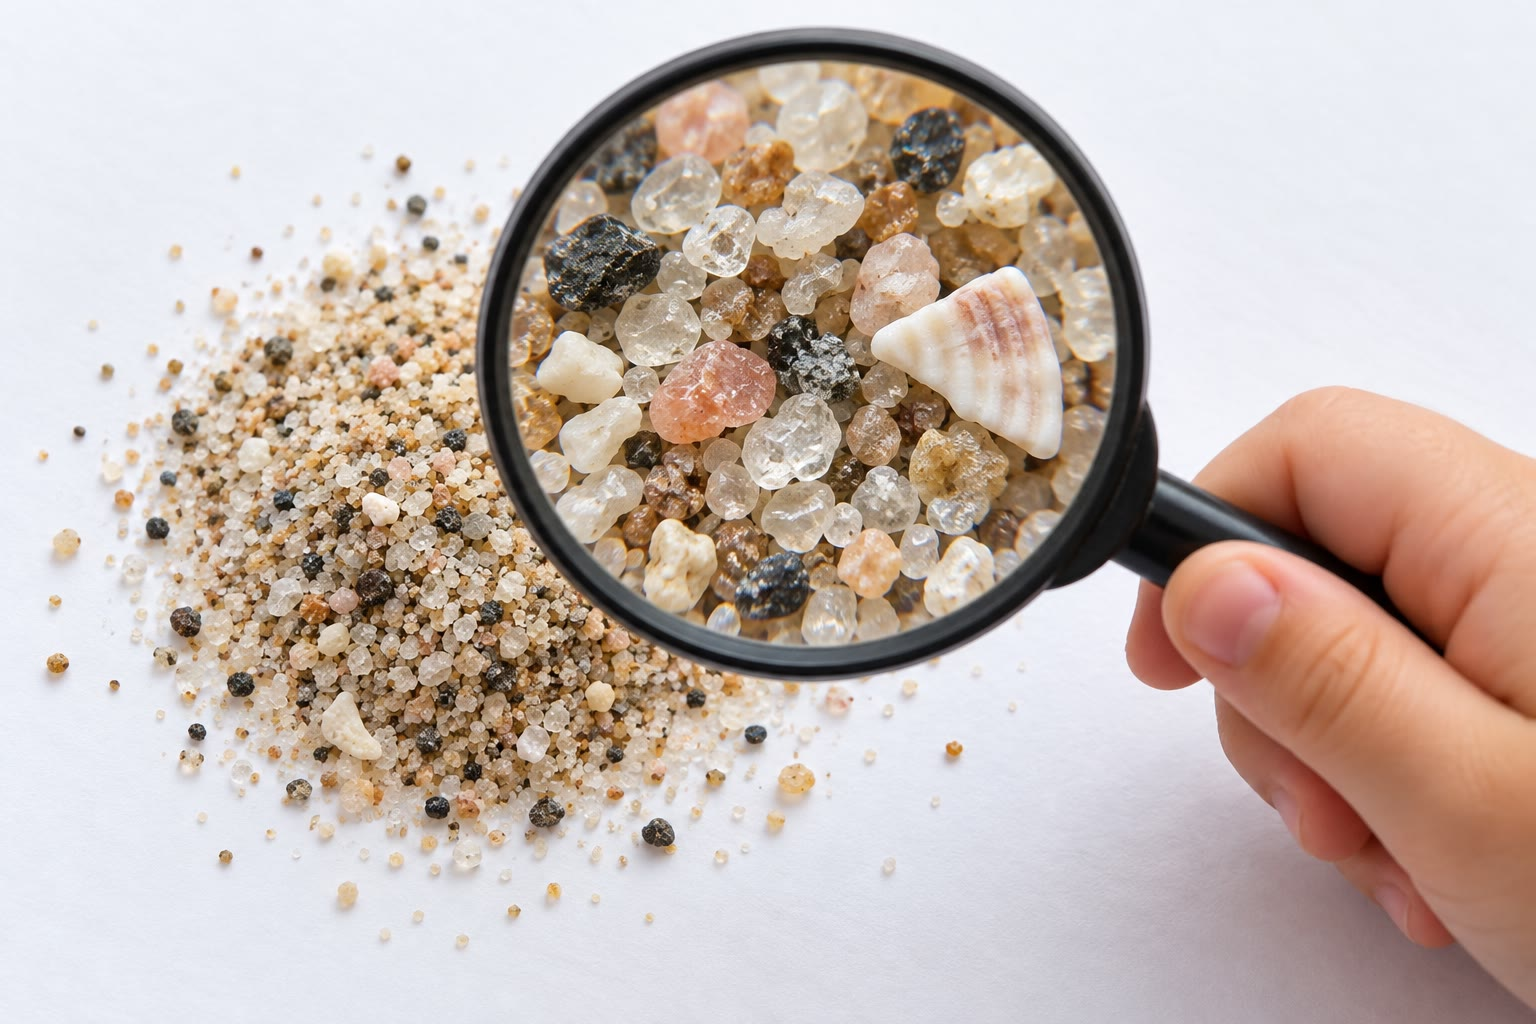
\includegraphics[width=0.55\linewidth]{images/book1/ai/g3-sand-magnifier.jpg}

{\small आवर्धक लेंस से दिखती \omterm{def:g2:water-on-earth:ocean}{समुद्र} \omterm{def:g1:landscapes-around-us:water}{तट} की \omterm{def:g3:stones-pebbles-sand:sand}{रेत}: \omterm{def:g3:stones-pebbles-sand:rock}{चट्टान} के नन्हे कण और सीपों के
टुकड़े।}
\end{omfigure}

\begin{method}[टूटी चट्टान को आकार के हिसाब से छाँटना]\label{met:g3:stones-pebbles-sand:sort}
टूटी \omterm{def:g3:stones-pebbles-sand:rock}{चट्टान} के किसी टुकड़े का नाम बताने के लिए उसका आकार देखो:
\begin{enumerate}
  \item अगर पास से देखने पर भी कण नहीं दिखते, तो वह \omterm{def:g3:stones-pebbles-sand:sand}{कीचड़} है;
  \item अगर हर कण दिखता है, पर हर एक 2 मिलीमीटर (एक सिक्के की मोटाई) से
        छोटा है, तो वह \omterm{def:g3:stones-pebbles-sand:sand}{रेत} है;
  \item अगर टुकड़े उससे बड़े हैं, पर एक टुकड़ा तुम हाथ में पकड़ सकते हो, तो वे
        \omterm{def:g3:stones-pebbles-sand:pebble}{बजरी} और \omterm{def:g3:stones-pebbles-sand:pebble}{कंकड़} हैं;
  \item अगर कोई टुकड़ा इतना भारी है कि उठाया न जा सके, तो वह शिलाखंड है।
\end{enumerate}
\end{method}

\begin{example}[हर आकार कहाँ मिलता है?]\label{ex:g3:stones-pebbles-sand:where}
तेज़ बहता पानी बड़े पत्थर ले जा सकता है; धीमा पानी उन्हें गिरा देता है और
सिर्फ़ छोटे कण ले जाता है। इसलिए शिलाखंड और नुकीले पत्थर खड़ी ढलान वाले
\omterm{def:g1:landscapes-around-us:landform}{पहाड़ी} नालों में पड़े रहते हैं; \omterm{def:g3:stones-pebbles-sand:pebble}{कंकड़} और \omterm{def:g3:stones-pebbles-sand:pebble}{बजरी} \omterm{def:g1:landscapes-around-us:landform}{घाटी} में \omterm{def:g1:landscapes-around-us:water}{नदी} के किनारों पर;
\omterm{def:g3:stones-pebbles-sand:sand}{रेत} \omterm{def:g2:water-on-earth:ocean}{समुद्र} तटों पर और \omterm{def:g1:landscapes-around-us:water}{नदी} के शांत मोड़ों में जमा होती है; और \omterm{def:g3:stones-pebbles-sand:sand}{कीचड़} वहाँ बैठता
है जहाँ पानी लगभग ठहरा हुआ हो, जैसे तालाबों, \omterm{def:g1:landscapes-around-us:water}{झीलों} और \omterm{def:g1:landscapes-around-us:water}{नदियों} के मुहानों में।
\end{example}

\section{कठोर चट्टानें और नरम चट्टानें}

सारी \omterm{def:g3:stones-pebbles-sand:rock}{चट्टानें} बराबर कठोर नहीं होतीं। कुछ, जैसे ग्रेनाइट, इतनी कठोर होती हैं
कि वे काँच पर खरोंच डाल देती हैं और दीवार में हज़ारों साल टिकी रहती हैं।
दूसरी हाथ में भुरभुरा जाती हैं, जैसे खड़िया, जो बोर्ड पर सफ़ेद निशान छोड़ती
है। कुछ \omterm{def:g3:stones-pebbles-sand:rock}{चट्टानें} ऐसे कणों से बनी हैं जो हमें दिखते हैं; दूसरी चिकनी होती हैं
और एक सिरे से दूसरे सिरे तक एक जैसी दिखती हैं।

\begin{example}[तीन चट्टानों की तुलना]\label{ex:g3:stones-pebbles-sand:three}
\emph{ग्रेनाइट} पर गुलाबी, सफ़ेद और काले कणों की चित्तियाँ होती हैं और वह
बहुत कठोर होता है। \emph{बलुआ पत्थर} आपस में चिपके \omterm{def:g3:stones-pebbles-sand:sand}{रेत} के कणों से बना है;
उँगली से रगड़ने पर कभी-कभी वह कुछ कण छोड़ देता है। \emph{खड़िया} सफ़ेद, नरम
और चूर्ण जैसी होती है। इनमें से हर एक कैसे बना, यह तुम आगे की किसी कक्षा में
सीखोगे।
\end{example}

\begin{omfigure}
\begin{tikzpicture}[font=\small]
  % three stones seen through a magnifying glass (drawn, not to scale)
  % granite: interlocking grains of three colours
  \begin{scope}
    \clip (0,0) circle (1.5);
    % a jittered lattice: the cells tile the disk with no gap, like the
    % interlocking crystals of granite
    \foreach \i in {-6,...,5} \foreach \j in {-6,...,5} {
      \pgfmathtruncatemacro{\c}{mod(abs(37*\i+17*\j+\i*\j),7)}
      \ifcase\c \def\col{pink!70}\or\def\col{pink!45}\or\def\col{white}\or
        \def\col{black!12}\or\def\col{white}\or\def\col{black!80}\else\def\col{pink!60}\fi
      \fill[\col, draw=black!35, line width=0.3pt]
        ({0.27*\i+0.07*sin(90*\i+131*\j)},{0.27*\j+0.07*cos(77*\i+61*\j)}) --
        ({0.27*(\i+1)+0.07*sin(90*(\i+1)+131*\j)},{0.27*\j+0.07*cos(77*(\i+1)+61*\j)}) --
        ({0.27*(\i+1)+0.07*sin(90*(\i+1)+131*(\j+1))},{0.27*(\j+1)+0.07*cos(77*(\i+1)+61*(\j+1))}) --
        ({0.27*\i+0.07*sin(90*\i+131*(\j+1))},{0.27*(\j+1)+0.07*cos(77*\i+61*(\j+1))}) -- cycle;
    }
  \end{scope}
  \draw[black!70, line width=2pt] (0,0) circle (1.5);
  \node at (0,-1.9) {ग्रेनाइट};
  \node[font=\scriptsize, align=center] at (0,-2.45) {तीन रंगों के बड़े कण,\\एक-दूसरे में फँसे};
  % sandstone: rounded grains touching
  \begin{scope}[xshift=4.2cm]
    \clip (0,0) circle (1.5);
    \fill[brown!45] (-1.6,-1.6) rectangle (1.6,1.6);
    \foreach \x in {-1.5,-1.1,...,1.6} \foreach \y in {-1.5,-1.15,...,1.6}
      \fill[yellow!50!brown!70, draw=brown!70!black, line width=0.3pt]
        ({\x+0.08*sin(97*\x+61*\y)},{\y+0.07*cos(53*\x-89*\y)}) circle ({0.16+0.03*sin(71*\x*\y)});
  \end{scope}
  \draw[black!70, line width=2pt] (4.2,0) circle (1.5);
  \node at (4.2,-1.9) {बलुआ पत्थर};
  \node[font=\scriptsize, align=center] at (4.2,-2.45) {आपस में चिपके\\रेत के गोल कण};
  % chalk: smooth, no grains to see
  \begin{scope}[xshift=8.4cm]
    \fill[white] (0,0) circle (1.5);
  \end{scope}
  \draw[black!70, line width=2pt] (8.4,0) circle (1.5);
  \node at (8.4,-1.9) {खड़िया};
  \node[font=\scriptsize, align=center] at (8.4,-2.45) {सफ़ेद और चिकनी: उसके कण\\इतने छोटे कि दिखते नहीं};
\end{tikzpicture}

{\small आवर्धक लेंस से देखी गई तीन \omterm{def:g3:stones-pebbles-sand:rock}{चट्टानें} (चित्र बनाया गया है)। ग्रेनाइट और
बलुआ पत्थर के कण दिखते हैं; खड़िया हर जगह एक जैसी दिखती है।}
\label{fig:g3:stones-pebbles-sand:magnified}
\end{omfigure}

\begin{method}[पत्थर को पास से देखना]\label{met:g3:stones-pebbles-sand:look}
किसी पत्थर का वर्णन करने के लिए, उसे तोड़े बिना, देखो और छूकर परखो:
\begin{enumerate}
  \item उसका रंग, या उसके रंग;
  \item उसका आकार: कोनों वाला नुकीला, या गोल और चिकना;
  \item उसके कण: क्या वे दिखते हैं? क्या सब एक जैसे हैं, या कई रंगों के?
  \item छूने पर कैसा लगता है: कठोर, या इतना नरम कि काग़ज़ पर निशान छोड़ दे?
\end{enumerate}
जो दिखे, उसे एक सारणी में लिखो, हर पत्थर के लिए एक पंक्ति।
\end{method}

\begin{example}[तीन पत्थरों की सारणी]\label{ex:g3:stones-pebbles-sand:table}
मिया स्कूल के एक डिब्बे से तीन पत्थरों का वर्णन करती है।
\begin{center}\small
\begin{tabular}{llll}
\hline
पत्थर & रंग & आकार & कण \\
\hline
A & गुलाबी, सफ़ेद और काला & गोल & बड़े, तीन रंगों के \\
B & पीला-भूरा & नुकीला & छोटे, सब एक जैसे \\
C & सफ़ेद & नुकीला & दिखते नहीं \\
\hline
\end{tabular}
\end{center}
पत्थर C काग़ज़ पर सफ़ेद निशान भी छोड़ता है। ऊपर के उदाहरण से पत्थर A
ग्रेनाइट जैसा लगता है, पत्थर B बलुआ पत्थर जैसा और पत्थर C खड़िया जैसा।
पत्थर A गोल है: पानी ने उसे बहुत समय तक लुढ़काया है।
\end{example}

\section{वे पत्थर जिनसे हम बनाते हैं}

हज़ारों सालों से लोग अपने आसपास की \omterm{def:g3:stones-pebbles-sand:rock}{चट्टान} से निर्माण करते आए हैं। किसी
इलाक़े के पुराने गाँवों में दीवारें अक्सर एक ही रंग की होती हैं, क्योंकि वे
सबसे पास की \omterm{def:g1:landscapes-around-us:landform}{पहाड़ी} के पत्थर से बनी थीं।

\begin{definition}[इमारती पत्थर]\label{def:g3:stones-pebbles-sand:building-stone}
\emph{इमारती पत्थर}\index{इमारती पत्थर} ऐसी \omterm{def:g3:stones-pebbles-sand:rock}{चट्टान} है जिसे दीवारें, छतें,
सीढ़ियाँ, पुल या फ़र्श बनाने के लिए काटा या गढ़ा जाता है।
\end{definition}

हर \omterm{def:g3:stones-pebbles-sand:rock}{चट्टान} किसी काम की होती है। कठोर ग्रेनाइट से ऐसी दीवारें, सीढ़ियाँ और
फ़ुटपाथ के किनारे बनते हैं जो सदियों तक टिकते हैं। कुछ \omterm{def:g3:stones-pebbles-sand:rock}{चट्टानें}, जैसे
स्लेट, पतली, चपटी परतों में फट जाती हैं: एक के ऊपर एक बिछाने पर वे ऐसी छतें
बनाती हैं जिनमें से बारिश अंदर नहीं आती। बलुआ पत्थर और चूना पत्थर इतने नरम
होते हैं कि उन्हें सुघड़ ब्लॉकों में काटा जा सके।

\begin{omfigure}
\begin{minipage}[b]{0.49\linewidth}\centering
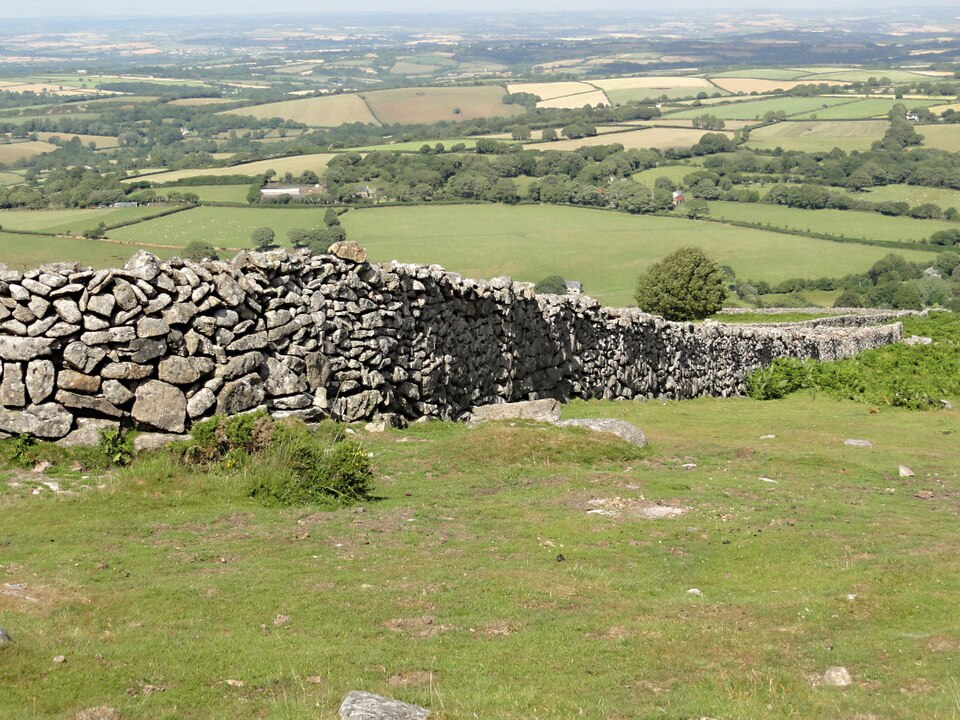
\includegraphics[width=\linewidth]{images/book1/g3-granite-wall.jpg}

{\small ग्रेनाइट के ब्लॉकों की दीवार, जिसे गारे के बिना बनाया गया है। चित्र:
टोनी एटकिन, जियोग्राफ़ (CC BY-SA 2.0)।}
\end{minipage}\hfill
\begin{minipage}[b]{0.49\linewidth}\centering
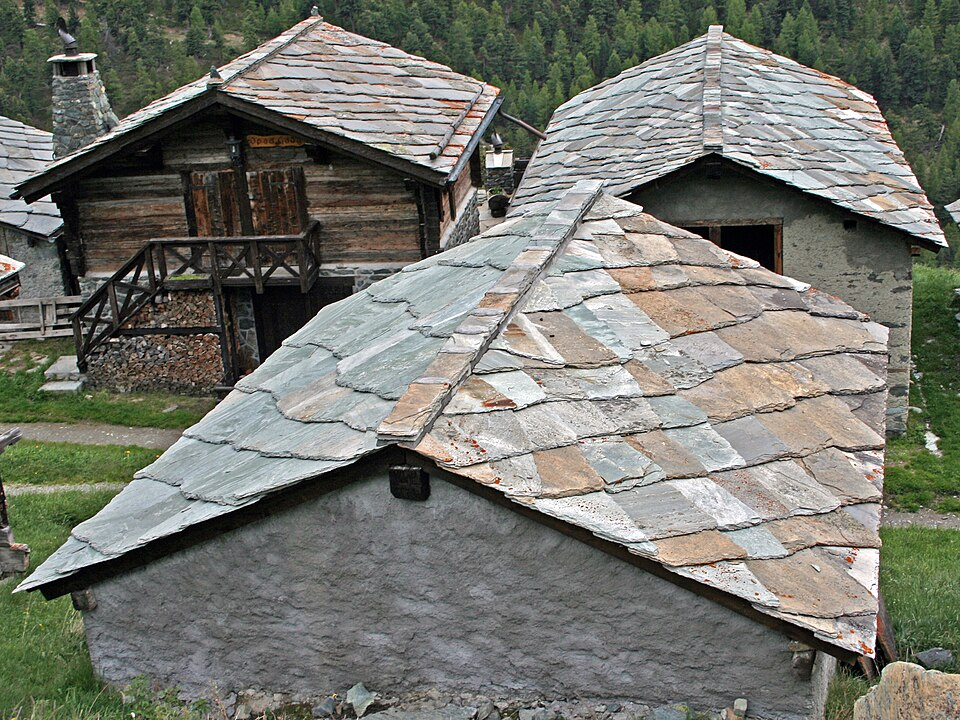
\includegraphics[width=\linewidth]{images/book1/g3-slate-roof.jpg}

{\small स्विट्ज़रलैंड के एक \omterm{def:g1:landscapes-around-us:landform}{पहाड़ी} गाँव में पत्थर की पतली, चपटी पटियों की छतें।
चित्र: माइकल सी.~राइगल (CC BY-SA 3.0)।}
\end{minipage}
\end{omfigure}

\begin{omfigure}
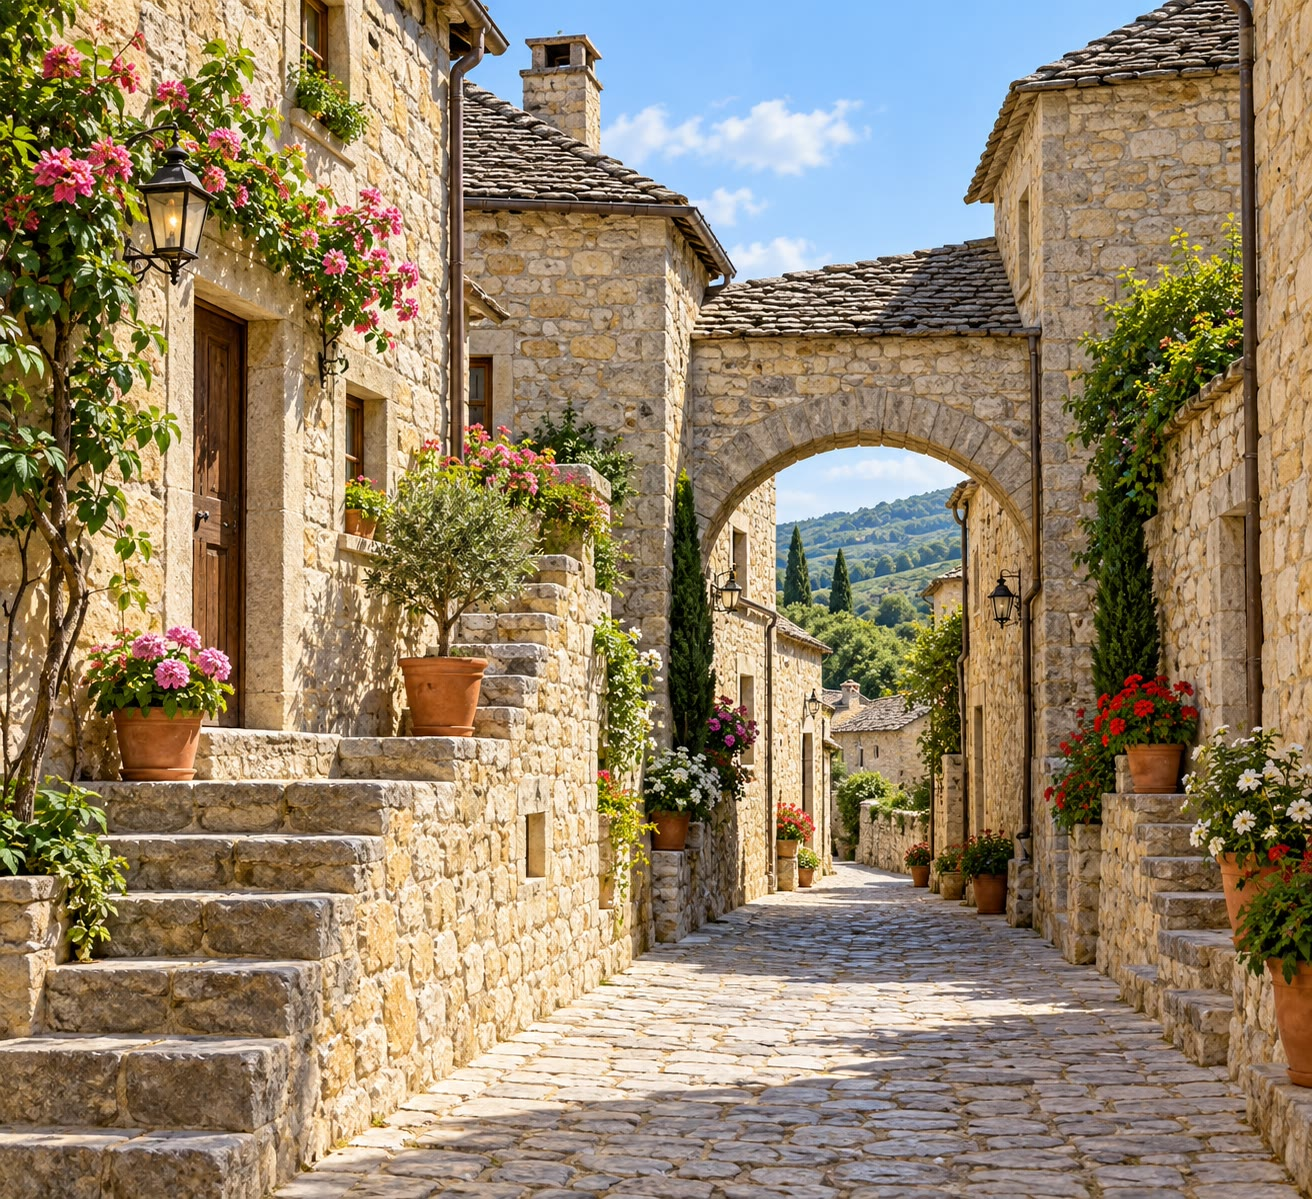
\includegraphics[width=0.6\linewidth]{images/book1/ai/g3-stone-village.jpg}

{\small पास की \omterm{def:g1:landscapes-around-us:landform}{पहाड़ी} के पत्थर से पूरा-का-पूरा बना एक पुराना गाँव।}
\end{omfigure}

आज हम ईंटों, कंक्रीट और काँच से भी बनाते हैं। पर ईंट पकाई गई मिट्टी से बनती
है, कंक्रीट \omterm{def:g3:stones-pebbles-sand:sand}{रेत}, \omterm{def:g3:stones-pebbles-sand:pebble}{बजरी} और सीमेंट से, और काँच \omterm{def:g3:stones-pebbles-sand:sand}{रेत} से: ये सब भी पृथ्वी की
\omterm{def:g3:stones-pebbles-sand:rock}{चट्टानों} से ही आते हैं।

\section{अभ्यास}

\begin{exercise}[$\star$]\label{exo:g3:stones-pebbles-sand:1}
\omterm{def:g3:stones-pebbles-sand:rock}{आधार चट्टान} क्या है? बिना खोदे हम उसे कहाँ देख सकते हैं?
\end{exercise}

\begin{exercise}[$\star$]\label{exo:g3:stones-pebbles-sand:2}
आकार के क्रम में लगाओ, सबसे छोटे से सबसे बड़े तक: \omterm{def:g3:stones-pebbles-sand:pebble}{कंकड़}, \omterm{def:g3:stones-pebbles-sand:sand}{कीचड़}, शिलाखंड,
\omterm{def:g3:stones-pebbles-sand:sand}{रेत}।
\end{exercise}

\begin{exercise}[$\star$]\label{exo:g3:stones-pebbles-sand:3}
एक कण 1 मिलीमीटर चौड़ा है। वह \omterm{def:g3:stones-pebbles-sand:sand}{रेत} है या \omterm{def:g3:stones-pebbles-sand:pebble}{बजरी}? एक और कण 3 मिलीमीटर चौड़ा
है: \omterm{def:g3:stones-pebbles-sand:sand}{रेत} या \omterm{def:g3:stones-pebbles-sand:pebble}{बजरी}?
\end{exercise}

\begin{exercise}[$\star$]\label{exo:g3:stones-pebbles-sand:4}
प्राकृतिक या लोगों का बनाया? एक \omterm{def:g3:stones-pebbles-sand:pebble}{कंकड़}; एक ईंट; ग्रेनाइट का एक ब्लॉक; काँच
की एक शीट; \omterm{def:g2:water-on-earth:ocean}{समुद्र} \omterm{def:g1:landscapes-around-us:water}{तट} की \omterm{def:g3:stones-pebbles-sand:sand}{रेत}।
\end{exercise}

\begin{exercise}[$\star$]\label{exo:g3:stones-pebbles-sand:5}
\omterm{def:g1:landscapes-around-us:water}{नदी} के \omterm{def:g3:stones-pebbles-sand:pebble}{कंकड़} में नुकीले कोने क्यों नहीं होते?
\end{exercise}

\begin{exercise}[$\star$]\label{exo:g3:stones-pebbles-sand:6}
दो \omterm{def:g3:stones-pebbles-sand:building-stone}{इमारती पत्थरों} के नाम बताओ, और बताओ कि इस अध्याय की तस्वीरों में हर एक
किस काम आया है।
\end{exercise}

\begin{exercise}[$\star\star$]\label{exo:g3:stones-pebbles-sand:7}
टॉम को एक ही \omterm{def:g3:stones-pebbles-sand:rock}{चट्टान} के दो पत्थर मिलते हैं: एक नुकीला है, दूसरा गोल। किसने
ज़्यादा लंबी यात्रा की है? समझाओ।
\end{exercise}

\begin{exercise}[$\star\star$]\label{exo:g3:stones-pebbles-sand:8}
कणों के आकार वाले चित्र में सबसे बड़ा \omterm{def:g3:stones-pebbles-sand:pebble}{कंकड़} कितने सेंटीमीटर लंबा है?
2 मिलीमीटर के \omterm{def:g3:stones-pebbles-sand:sand}{रेत} के कितने कण 1 सेंटीमीटर में एक-दूसरे से सटाकर रखे जा
सकते हैं?
\end{exercise}

\begin{exercise}[$\star\star$]\label{exo:g3:stones-pebbles-sand:9}
तुम्हें \omterm{def:g3:stones-pebbles-sand:sand}{कीचड़} कहाँ मिलने की उम्मीद होगी: किसी तेज़ \omterm{def:g1:landscapes-around-us:landform}{पहाड़ी} नाले में या किसी
शांत तालाब में? क्यों?
\end{exercise}

\begin{exercise}[$\star\star$]\label{exo:g3:stones-pebbles-sand:10}
ईंटें, कंक्रीट और काँच लोग बनाते हैं। फिर भी हम क्यों कह सकते हैं कि वे
पृथ्वी की \omterm{def:g3:stones-pebbles-sand:rock}{चट्टानों} से आते हैं?
\end{exercise}
